\section{Machine Translation}
\begin{itemize}
	\item \textcolor{red}{THINK ABOUT WHAT TO PUT IN HERE}
\end{itemize}
\subsection{Statistical Machine Translation}
\begin{itemize}
	\item Given a sentence $f$ in foreign language, find most probable translation $\hat{e}$:
	$$\hat{e} = \arg\max_{e} P(e|f) = \arg\max_{e} \underbrace{P(f|e)}_{\text{channel}} \underbrace{P(e)}_{\text{source}}$$
	\item The source is the \textbf{language model} which makes sure that the grammatical structure in the text is correct
	\begin{itemize}
		\item It is also helpful for disambiguate the word decision in the translating language
		\item This is very important if a word in the foreign language is ambiguous
	\end{itemize}
	\item The (noisy) channel is the \textbf{translation model} which is responsible to translate the text (makes sure that $f$ are translations of $e$)
	\item IBM-3 model:
	\begin{itemize}
		\item For every word:
		\begin{itemize}
			\item Choose a fertility $\phi_i$ (number of words in goal language should be translated into in foreign language. E.g. ``did'' has fertility of 0, ``slap'' 3 in French)
			\item Generate $\phi_i$ foreign words
			\item Generate spurious/default words that might be needed
		\end{itemize}
		\item Permute translated words based on the position a word was before, and language it was in before
	\end{itemize}
\end{itemize}
\subsubsection{Learning parameters of models}
\begin{itemize}
	\item For learning the parameters of the language and translation model, we would need the word alignments in the translation which however require the parameters
	\item Thus, we apply the Expectation-Maximization algorithm
	\item Assume we have alignments, but for every sentences multiple ones. For example, we can have the following possible alignments for a two-word sentence:
	\begin{figure}[ht]
		\centering
		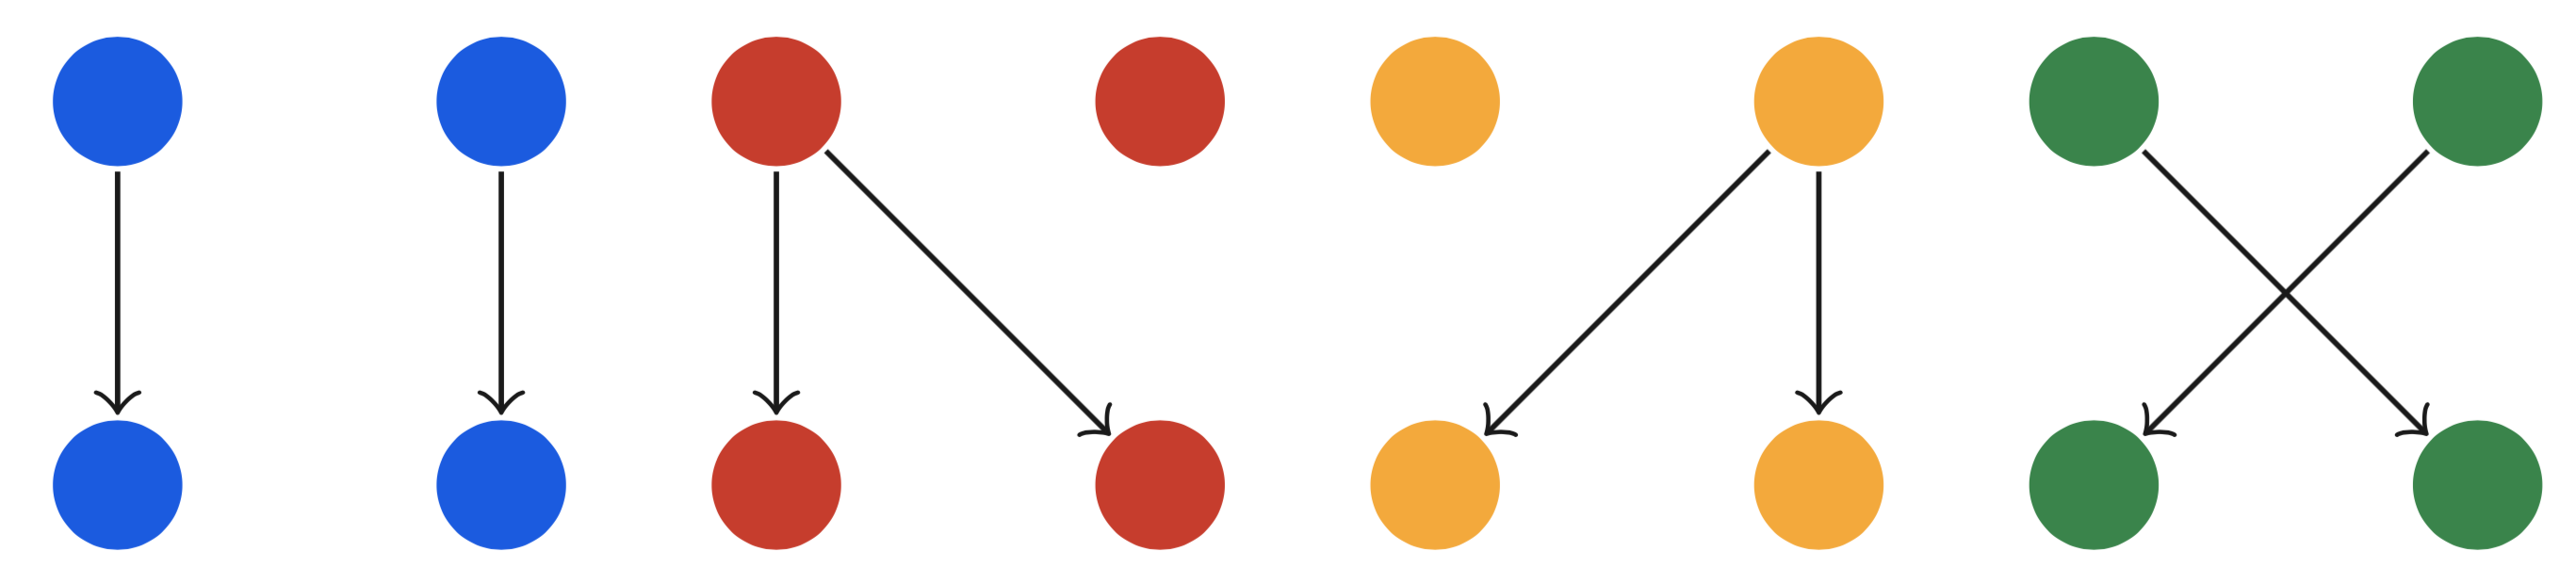
\includegraphics[width=0.5\textwidth]{figures/translation_EM_alignment.png}
	\end{figure}
	\item Every alignment is assigned to a probability/fractional count it occurs. Initially, we set the probability of every alignment/word to a uniform distribution
	\item We try to maximize the probability that a foreign word/phrase $f_j$ in our corpus is  a translation of $e_{a_j}$ where $a_j$ is the alignment of the foreign to translated language. When using Bayes rule (and looking at only 1to1 alignments), we maximize:
	$$P(a,f|e) = \prod\limits_{j=1}^{M}t(f_j|e_{a_j})$$
	where $t$ are the fractional counts
	\item EM algorithm:
	\begin{enumerate}[label=Step \theenumi:]
		\item Compute $P(a,f|e)$ for every possible alignment and sentence
		\item Normalize the alignments for the same foreign sentence. $P(a,f|e)\to P(a|f,e)$
		\item Collect the fractional counts $tc(x|b)$ by summing up the probabilities of all $P(a|f,e)$ where $b$ is aligned to $x$. 
		\item Normalize fractional counts by $b$ $\Rightarrow$ revised parameters for next iteration
	\end{enumerate}
	\item Example: Given $t(x|b) = 1/4$, $t(x|c)= 3/4$, $t(y|b)= 1/2$, $t(y|c)= 1/2$.
	\begin{figure}[ht]
		\centering
		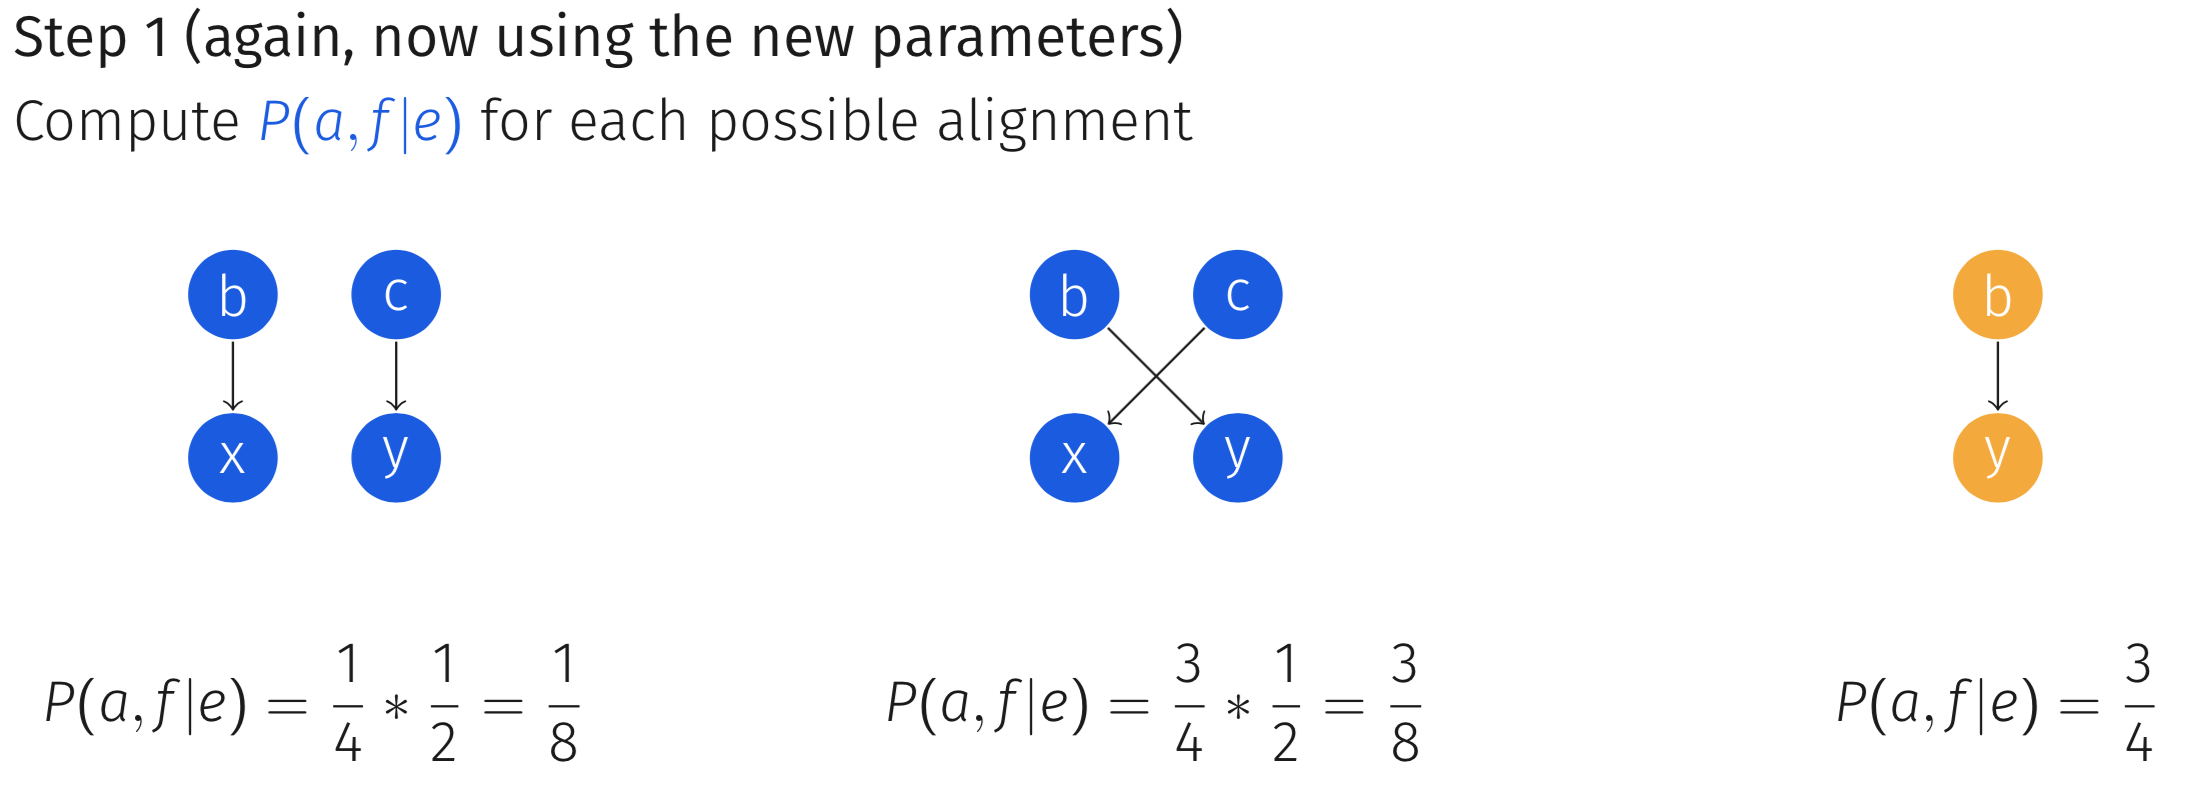
\includegraphics[width=0.5\textwidth]{figures/translation_EM_step_1.png}
	\end{figure}
	\begin{figure}[ht]
		\centering
		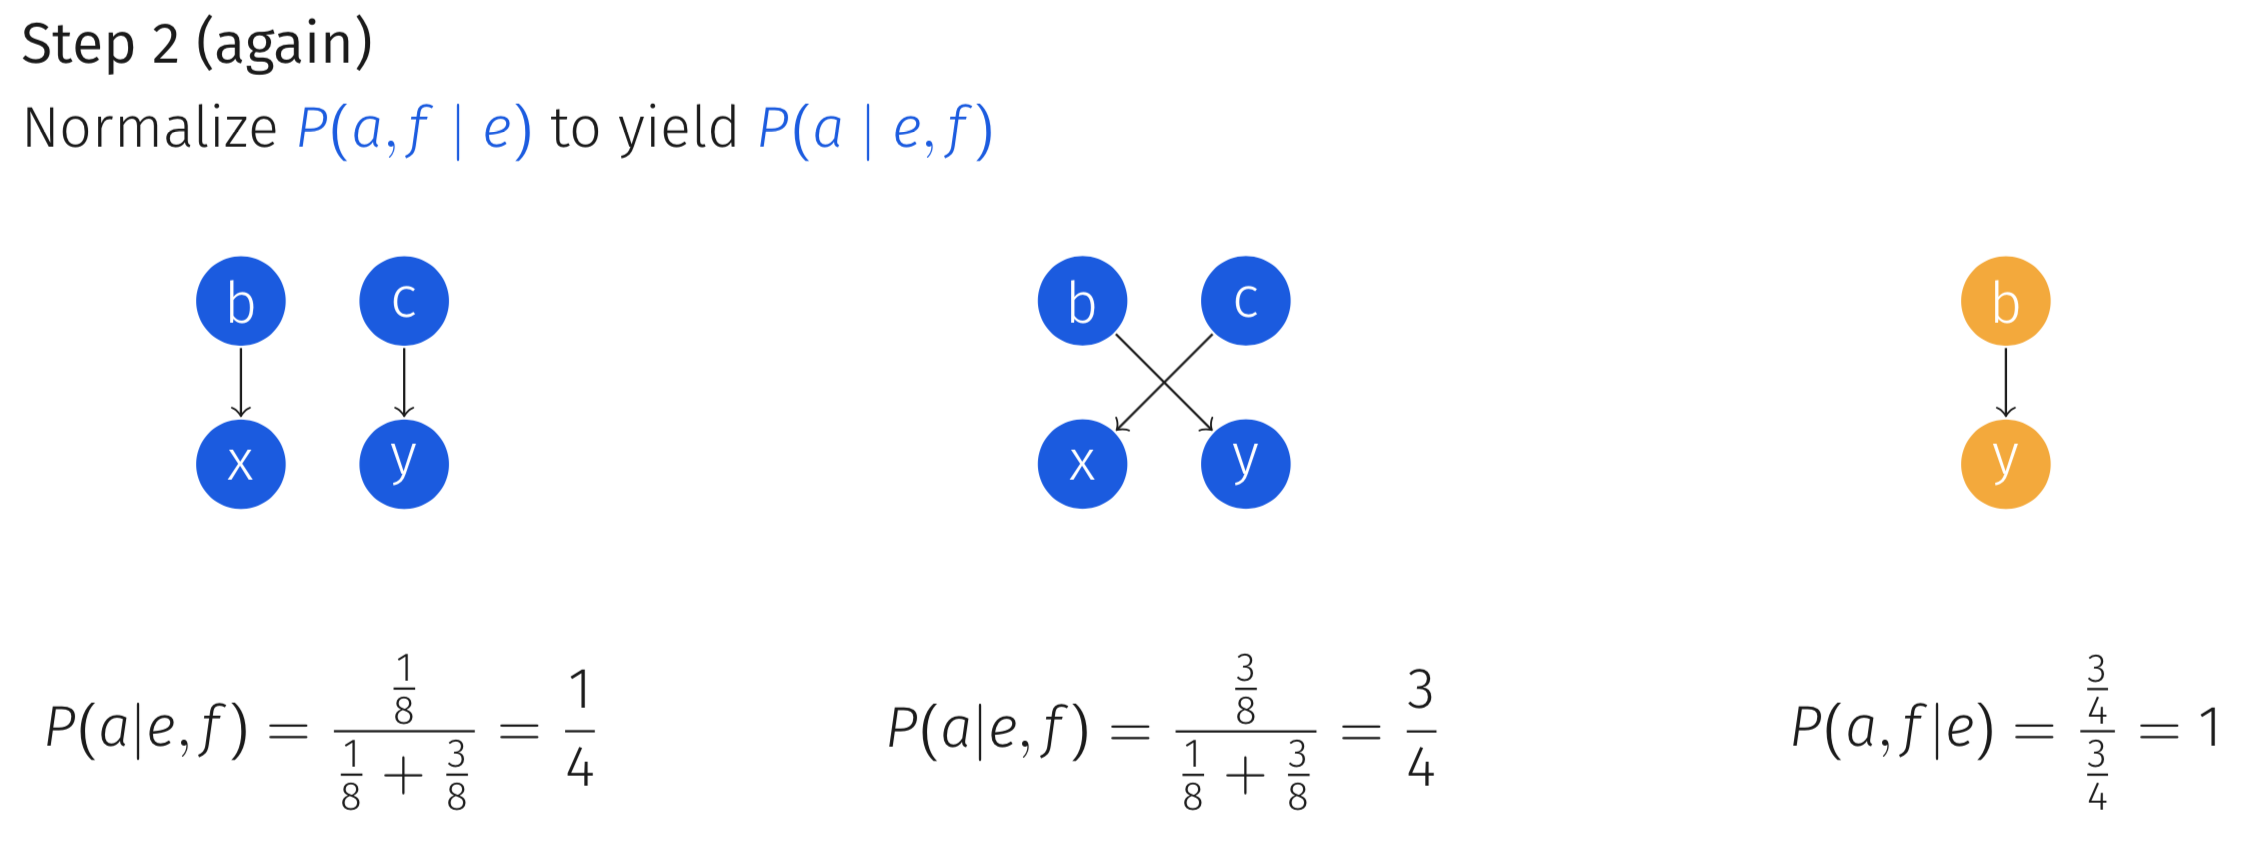
\includegraphics[width=0.5\textwidth]{figures/translation_EM_step_2.png}
	\end{figure}
	\begin{figure}[ht]
		\centering
		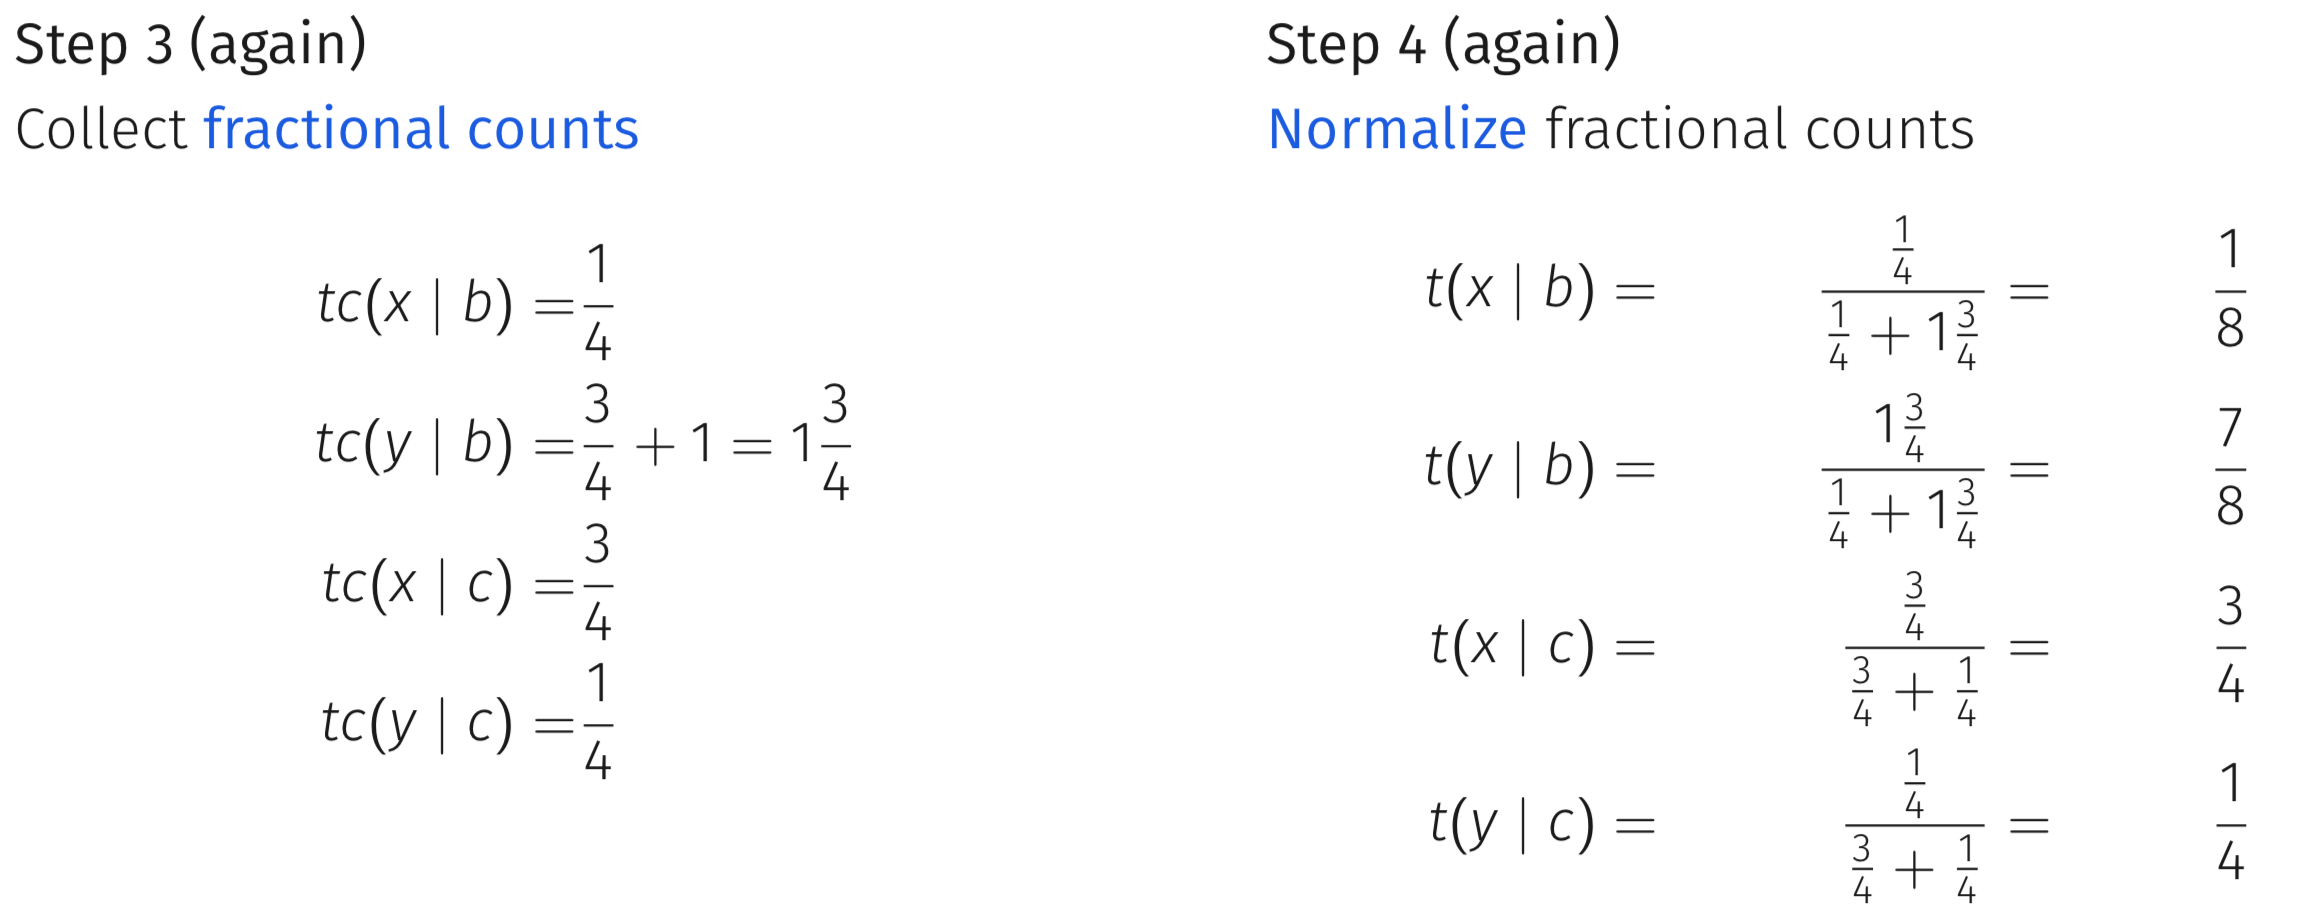
\includegraphics[width=0.5\textwidth]{figures/translation_EM_step_3_4.png}
	\end{figure}
	\item Note on EM: Optimization function is non-convex so that we might find a local minimum
\end{itemize}
\subsection{Phrase-based Statistical Machine Translation}
\begin{itemize}
	\item Previously, translation was based on single words as atomic unit. However, we can also use phrases (few consecutive words) as unit 
	\item The advantage is that context can be taken into account for translation, and no more fertility, insertion and deletion of words are necessary to translate
	\item We now have a phrase table where we have probabilities to translate a certain phrase into another
	\item The translation model uses phrases instead of words, but also needs to consider to reorder the phrases:
	$$P(f|e) = \prod\limits_{i=1} \phi(\overline{f}_i | \overline{e}_i) \underbrace{d(\text{start}_i - \text{end}_i -1)}_{\text{distance-based reordering}}$$
	Note that $\text{start}$ and $\text{end}$ are the positions in the foreign language, but $i$ is the index of the translated language!
	\item Extract all phrases that are consistent with a word alignment $A$. A phrase is consistent if all words of $\overline{f}'$ are only aligned to words in $\overline{e}'$ and not any other words outside this phrase (and the other way round).
	\item The \textit{phrase translation probability} $\phi$ is estimated by the relative frequency:
	$$\phi(\overline{f}, \overline{e}) = \frac{\text{count}(\overline{f}, \overline{e})}{\sum_i \text{count}(\overline{f}_i, \overline{e})}$$
\end{itemize}